\chapter{Discussion}

% This study aimed to generate multi-locus genetic barcoding data for the identification of the species and lineages within the \textit{Dactylopius} genus. Of particular interest were the lineages within \textit{Dactylopius opuntiae}, namely `ficus' and `stricta', used for the control of \textit{Opuntia ficus-indica} and \textit{Opuntia stricta}, respectively, and a number of \textit{D. tomentosus} lineages used for the control of invasive \textit{Cylindropuntia} species. Successful biological control programmes rely on the correct identification of control agents, as different species and intraspecific lineages can offer varying levels of control efficacy. The output of this project is thus highly valuable to programmes aimed at controlling invasive Cactaceae using \textit{Dactylopius} agents. \\
This chapter summarises and explains the results obtained from two mitochondrial regions, one nuclear gene region, and two ISSRs used to assess the identification accuracy of the Dactylopiidae using both tree-based methods and barcode testing algorithms. It also discusses aspects relating to geographical distribution, and the practical applications arising from this thesis.

\section{Genetic markers}
\subsection{12S}

The 12S rRNA genetic marker provided 100\% identification accuracy (IA) at both the species level (at a 1\% genetic distance threshold) and for three of the six \textit{D. tomentosus} lineages (at a 0.2\% genetic distance threshold) using barcode testing algorithms. Bayesian (BI) and Maximum Likelihood (ML) phylogenies supported this result, showing well-supported clades that distinguished all species. Both standard and secondary structure RNA alignment methods suggest that this marker can accurately distinguish between the `californica', `cholla', and `imbricata' lineages, but that the `echinocarpa x acanthocarpa', `bigelovii', and `cylindropuntia spp.' samples form one clade. \\
The BI tree showed a well-supported separation between South African and Australian \textit{D. ceylonicus} samples. This is most likely due to the fact that the species was released in South Africa and Australia in 1913 and 1914, respectively, and have been isolated from each other for more than a hundred years. The agents used in these two releases came from the same stock, which were originally collected in Brazil, then exported to India, and subsequently to Sri Lanka \citep{Winston2014BiologicalWeeds.}. \textit{Dactlopius austrinus} and \textit{D. tomentosus} `imbricata' and `cholla' did not show the same separation between the two countries, most likely because they have not been separated for long enough. \\ 
The 12S rRNA primers successfully amplified the target region of five of the six \textit{Dactylopius} species used in this project (only \textit{D. confertus} was unsuccessful), and had the highest mean between-group K2P distance (0.30 $\pm$ 0.14). The marker is not, however, useful for distinguishing between \textit{D. opuntiae} `ficus' and `stricta' lineages, due to the presence of negative barcode gaps (i.e. intraspecific variation $>$ interspecific variation) at that higher resolution taxonomic level. The BI tree aligned according to the secondary structure of RNA did not vary greatly from the standard alignment, but did show stronger support for a single clade containing the \textit{D. tomentosus} `echinocarpa x acanthocarpa' and `bigelovii' lineages that was separate from the `cylindropuntia sp.' samples.  \\
A number of other studies have found the 12S rRNA marker highly useful for DNA fingerprinting, such as for the identification of ticks (Acari: Ixodida) \citep{lv2014assessment}, earthworms (Lumbricidae) \citep{klarica2012comparing}, commercial fishes \citep{ardura2010dna, hardy2011dna, cawthorn2012evaluation}, snakes (from venom samples) \citep{pook2005mitochondrial}, and various animal species used in traditional medicines \citep{luo2011application}.
Based on the results of this study, and due to the ease of PCR amplification of the Dactylopiidae using this gene region, it is recommended as the most efficient for species-level identification, and for the identification of the `cholla', `californica', and `imbricata' lineages within the \textit{D. tomentosus} species.

\subsection{18S}
The 18S rRNA marker could accurately distinguish between all \textit{Dactylopius} species, except for \textit{D. austrinus} and \textit{D. ceylonicus}, which grouped into one clade and were the only two species with negative barcode gaps. This may suggest a more recent speciation event between these two species, relative to the others. The overall IA was 94.59\% at the species level. The primers successfully amplified the target region of all six \textit{Dactylopius} species used in this study. The genetic distance threshold for this marker was lower (0.2\%) for species level identification, and had the lowest mean between-group K2P distance (0.03 $\pm$ 0.02) owing to the slow evolutionary rate in this nuclear gene relative to mitochondrial regions. \citet{evans2007assessment}, for example, tested COI, rbcL, 18S and ITS rDNA as potential barcoding regions, and found that 18S was the least variable marker. \\
Of the \textit{D. tomentosus} lineages, only `cholla', and `echinocarpa x acanthocarpa' and `bigelovii' formed separate clades, while `imbricata', `californica', and `cylindropuntia' were unresolved. In their study of Murray-Darling Basin fishes, \citet{hardy2011dna} found that the 18S rRNA marker could successfully identify 83.1\% of the species sampled, but that there were a number of different species within a genus complex that shared identical sequences. In the study by \citet{Campana2015}, no intraspecific variation was found within the seven sequences obtained from \textit{D. coccus} populations. This corroborates the findings of the current project, namely that this marker is uninformative for identification beyond the species level. It can, however, be used for the inference of phylogenetic relationships between species, particularly when supplementing a concatenated genetic data set.

\subsection{COI}
COI-A primers could distinguish between \textit{D. confertus}, \textit{D. opuntiae}, and \textit{D. confusus} with a 100\% IA. A 1\% genetic distance threshold was found to be to be optimal for assessing identification accuracy at the species level, which is consistent with the barcoding literature \citep{Hebert2003, Hebert2003a}. It is not, however, able to distinguish between \textit{D. opuntiae} lineages. When barcode accuracy was tested at the lineage level, all \textit{D. opuntiae} sequences displayed negative barcode gaps (intraspecific variation $>$ interspecific variation) due to the high similarity between the `ficus' and `stricta' lineages. 
The average within-group p-distance was similar to that of the 12S region (0.22 $\pm$ 0.1). \\
COI-B primers successfully amplified all \textit{D. tomentosus} lineages. At a genetic distance threshold of 3.3\%, IA increased from 70.37\% to 100\% when the `echinocarpa x acanthocarpa', `bigelovii', and `cylindropuntia sp.' lineages were treated as one lineage. ISSR analyses for these particular lineages may reveal further differences between them. 

\section{Distance-based barcode testing}

In agreement with \citet{Birch2017TestingAustralia}, the TID barcode testing algorithm is the more conservative test, and is recommended as the most appropriate since it takes into consideration a genetic distance threshold. It, therefore, reduces the number of false positive identifications, as opposed to the NN and BCM tests. The NN algorithm was mostly an inappropriate measure in the context of this study, particularly with reference to the lineage level where genetic similarity was very high. 
% For example, the 12S marker showed a TID hit rate of only 13.04\% for \textit{D. opuntiae} lineages at a 0.2\% threshold, but the NN showed a 80.43\% accuracy rate. 
Since each gene evolves at a different rate, a one-size-fits-all approach of a default 1\% distance threshold is inaccurate. Combining appropriate distance and tree-based methods to determine barcoding accuracy offers a more thorough approach to the identification of target taxa.

\section{Posterior probabilities vs bootstrap values}

Some clades in the phylogenies in this study showed much higher bayesian posterior probability (BPP) support than their corresponding ML bootstrap values. This is not uncommon, and stems from the fact that these two methods assess data in fundamentally different ways and are based upon different statistical assumptions \citep{huelsenbeck2002potential, douady2003comparison, garcia2004comparison, huelsenbeck2004frequentist}. \citet{huelsenbeck2002potential} suggest that the ML bootstrap method underestimates the confidence of phylogenetic clades, and propose that a Bayesian analysis is the most easily interpretable and accurate given the correct evolutionary models. In a simulation, \citet{alfaro2003bayes} found that the greatest disparity between BPP and bootstrap values occurred when the branch lengths were short, or when the number of characters available for comparison was small. They suggest that a Bayesian analysis offers a greater sensitivity to phylogenetic signal, and that a substantial increase in the number of characters will facilitate the convergence of bootstrap values to BPP. \\ 
% The 12S sequences were the shortest of the four genetic markers, at $\sim$ 413 base pairs in length in the final alignment (compared to 18S with $\sim$ 570 base pairs, PCOF1 and LepR1 with $\sim$ 526 and DTOMf and HCO2198 with $\sim$ 546 base pairs). This could be a contributing factor to the differences in support values between the BI and ML trees. 
A study by \citet{hardy2011dna} used the 12S rRNA region (in addition to 18S rRNA and the mtDNA control region (CR)) to differentiate between different fish species in the Murray-Darling River Basin in Australia. The BI and ML analyses did not differ substantially in their support values, but they did report that the 12S trees in particular showed greater variability (where a number of clades had bootstrap support values $<$ 75 and BPP $>$ 95). Similarly, a study by \citet{wilcox2002phylogenetic} analysed the 12S, 16S, and valine-tRNA gene regions of dwarf boa snakes (Tropidophiidae), and found that some branches in their 12S and 16S phylogenies had BPP values more than double that of the corresponding bootstrap support values. Based on their results, the authors recommended the use of Bayesian analyses above bootstrapping methods, as it provided a more reliable estimation of phylogenetic accuracy. The present study supports this statement, especially taking into account the faster computational time that a Bayesian analysis offers compared to other methods \citep {huelsenbeck2001bayesian, douady2003comparison}.

\section{ISSR fragment analysis}
The percentage of polymorphism found in this study was lower than that reported by \citet{silva2013genetic}, who collected \textit{D. opuntiae} on \textit{O. ficus-indica} host plants in the native range in northeast Brazil. 
% For example, the present study reported a percentage polymorphism average of 22 and 38.53\% for `stricta' and `ficus', respectively, compared to the 71.4\% polymorphic loci for ISSR 809 ((AG)\textsubscript{8}C), and a maximum of 87.5\% for the TCT(GA)\textsubscript{7} primer reported in their study. 
Their overall polymorphism percentage was 70.9\%, taken as an average of nine different ISSR primers. The present study reported only 44.93\% polymorphism. Additionally, they reported a genetic similarity of 80\% across all populations. Comparatively, the present study reported an average Jaccard similarity of 51.67\% (SE $\pm$ 1.01) for all \textit{D. opuntiae} samples. This is arguably due to the higher number of fragments reported in the present study due to the use of DNA fragment analysis using capillary electrophoresis. Over three-fold more fragments were found per primer than by \citet{silva2013genetic}, who scored fragments manually through visualising bands on agarose gels. 
\citet{silva2013genetic} used both ISSR and RAPD primers to distinguish between \textit{D. opuntiae} populations, and concluded that the RAPD primers used were more effective than ISSRs in grouping populations, but neither method succeeded in discriminating between populations from different geographic regions. \\
The \textit{D. opuntiae} ISSR data using Bayesian and ordination methods showed a statistically significant difference between the `ficus' and `stricta' lineages that the traditional DNA gene regions failed to reveal. The methods also showed significant differences between \textit{D. opuntiae} `ficus' populations; namely wild populations collected on \textit{O. ficus-indica} and \textit{O. engelmannii} in the Eastern Cape, and specimens collected from \textit{O. ficus-indica} around the Uitenhage Mass Rearing Facility (MRF) and in Namibia. 

\subsection{`Stricta' and `ficus' lineages}

\subsubsection{Eastern Cape wild populations}
An unexpected result arising from the Bayesian Structure analysis (and supported by the nMDS ordination grouping) was that when forced into one of two cluster groups, the wild `ficus' populations collected from \textit{O. ficus-indica} and \textit{O. engelmannii} in the Eastern Cape were more genetically similar to the `stricta' cluster than they were to known `ficus' samples. It is possible that the wild populations have regularly hybridised with `stricta' and `ficus' lineages (hybridisation between these two lineages is reported in the work by \citet{Hoffmann2002BiologicalBiotypes} and  \citet{Hoffmann2004}), and that the genotypic status detected by the two specific ISSR primers used in this study currently aligns more with that of `stricta'. Collecting more specimens from \textit{O. ficus-indica} and \textit{O. engelmannii} in more distant regions of the country (in addition to the Namibian samples included in this study that grouped in the `ficus' cluster) could provide further clarity. When forced into one of five cluster groups, the wild populations did represent a distinct genotypic cluster not shared by any of the `stricta' genotypes. 


\subsubsection{Uitenhage Mass Rearing Facility (MRF)}
The \textit{D. opuntiae} population believed to be of the pure-bred `stricta' lineage at the MRF were more similar to `ficus' samples collected from \textit{O. ficus-indica} growing around the facility and from Namibian samples than they were to `stricta' samples. The MRF individuals are either the result of crosses between the two lineages, or they are merely part of the `ficus' group. This suggests that contamination has taken place, and that the control efficacy of the hybrid individuals being reared may be compromised. It is recommended that 1) the current culture be destroyed, and replaced with a new colony that is known to be the `stricta' lineage, 2) the wild `ficus' populations around the MRF should be killed, and 3) the genetic status of the colonies be checked on a regular basis to ensure that a pure-bred lineage is maintained. Additionally, it would be worth crossing and backcrossing the pure `stricta', `ficus', and MRF populations to test their host-specificities.

\subsubsection{The Kruger National Park and Saudi Arabia}
The \textit{D. opuntiae} samples from the Kruger National Park shared a genotypic cluster with the known `stricta' source populations (kept by Hildegard Klein and John Hoffmann), and were different from the `ficus' clusters. It could therefore be confirmed that these samples were of the `stricta' lineage. Similarly, the Saudi Arabian \textit{D. opuntiae} samples collected from \textit{O. stricta} shared a genetic cluster with the `stricta' source populations; confirming their identity as well. These populations can therefore effectively control \textit{O. stricta} \citep{githure1999host, Volchansky1999}, and can be mass reared if necessary. These populations can also be used as a source for the new clean culture of `stricta' at the Uitenhage MRF.

\subsection{ISSR identification accuracy}
Due to the different kind of data that ISSR analyses produce, the distance threshold required to create species group designations was much higher than that of nucleotide sequence data (60\% compared to the standard 1\%). This is because the latter is much more data-rich compared to binary information. \\
The identification success rate for \textit{D. opuntiae} lineages was 81.82\% at a 45\% distance threshold, with the remaining 18.18\% falling into the `No ID' category.  ISSR analysis using the methods described in this work offers a new and valuable tool to biological control efforts, as it allows practitioners to distinguish between these otherwise morphologically identical lineages. The \textit{D. tomentosus} lineages included in the ISSR analyses (`imbricata', `cholla', and `californica') showed a 100\% IA at a distance threshold of 45\%, although using the 12S rRNA marker to identify these is less labour intensive. \\
Of the two ISSR primers used, ISSR 826 had an average Jaccard error rate 5\% greater than ISSR 809, and tended to be less informative for some population groups compared to the latter primer. The average Euclidean error rates of 0.08 ($\pm$ 0.03) and 0.09 ($\pm$ 0.03) for ISSR 809 and ISSR 826, respectively, were in the same range as that found by \citet{paterson2013issrs} for \textit{Chromolaena odorata}. Whether the shared absence of bands is included in the error rate calculation can greatly impact its interpretation, and so it is important that future studies include both the Euclidean and Jaccard error rates for comparison. The present study reported average Jaccard error rates 6-fold greater than their Euclidean equivalent, which is comparable to those found by \citet{holland2008optimizing}, who reported a 4-fold difference in one experiment. \\
Although a 81.82\% hit rate is high for the identification of \textit{D. opuntiae} lineages, there are a multitude of other ISSR primers that may offer lower error rates and amplify a larger number of fragments. It would be worth using capillary electrophoresis to test the TCT(GA)\textsubscript{7} ISSR primer reported by \citet{silva2013genetic} as producing the highest percentage of polymorphic loci, and to test the RAPD primers used in their study.

% \subsection{Australian \textit{D. tomentosus} lineages}
% Both the 12S rRNA and COI (DTOMf \& HCO2198) markers clearly distinguished between the `californica', `cholla' and `imbricata' lineages, and showed that the `echinocarpa x acanthocarpa' and `bigelovii' lineages grouped into one clade due to their high level of genetic similarity. Support for the `cylindropuntia sp.' samples forming their own distinct clade was ambiguous. There is more support for them forming part of the `echinocarpa x acanthocarpa'/bigelovii' clade. ISSR analyses may offer further resolution in this case.

\section{Geographical distribution}
The first phylogeny for the Dactylopiidae was constructed by \citet{Perez-Guerra1992} using morphological data. The authors concluded that all the \textit{Dactylopius} species derived from one common ancestor, that \textit{D. coccus} was the most basal species, and that \textit{D. ceylonicus} was the most derived. \citet{Rodriguez2001} later created a phylogeny based on both morphological traits and geographical distributions, which formed two clades separating North and South American species. The results from the present study, and those from a molecular analysis by \citet{Ramirez-Puebla2010MolecularBacteria} (using the same 12S and 18S genetic markers), did not find this well-defined separation between the northern and southern continents (Fig. \ref{fig:phylogeny_comparison}). 
Both studies did, however, agree with the finding that \textit{D. tomentosus} was the most different from the other species. This is expected, because \textit{D. tomentosus} has a considerably different life history and morphological characteristics \citep{Perez-Guerra1992, Mathenge2009}.
The present results also agree with \citet{Rodriguez2001}'s finding that \textit{D. austrinus} and \textit{D. ceylonicus} are very closely related. These are both South American species. \\
Conflicting results between morphological phylogenies have been reported for this genus \citep{Portillo2006AENEMIES}, and  numerous other studies have reported on what is termed the `morphological-molecular conflict' \citep{cohen2018match}. Morphological phylogenies can be misleading due to the convergent evolution of traits, as homologous morphologies are not necessarily the result of homologous genes \citep{cartmill1994critique}. \citet{cohen2018match}, for example, states that \textit{ `morphological characters are only indirectly genealogical...and are intrinsically not capable of reporting evolutionary history'}. \\
The absence of a clear north-south geographic divide between the Dactylopiidae species is not unexpected, since the Cactaceae evolved in South America about 65 mya (some studies have suggested ranges between 100 \citep{mauseth1990continental} and 30 mya \citep{hershkovitz1997evolutionary}) following the Gondwana split, and only later dispersed northwards \citep{Anderson2001}. The North and South American continents were only connected by land (the Isthmus of Panama) about 5.7 mya, and so dispersal to the north prior to that is debatable \citep{Anderson2001, portillo2007biogeography}.
It is possible that some cacti dispersed via island bridges formed by the Central American Volcanic Arc, and rafting prior to the land connection \citep{Anderson2001}, and it has also recently been proposed that the Isthmus of Panama may have in fact formed 13 to 10 mya \citep{montes2015middle}. Thus the palaeontological event known as the `Great American Biotic Interchange' (GABI) may have occurred much earlier; although these are only hypotheses. \\
Based on the particular gene regions used in this study, which are also supported by the findings of \citet{Ramirez-Puebla2010MolecularBacteria}, it may be that there were multiple dispersal events of the Dactylopiidae from South to North America at different times. And that these founder populations proceeded to speciate in North America.
This raises interesting questions around the coevolution between the Cactaceae and the Dactylopiidae, and the role that human-mediated dispersal had to play in the insects' current distribution.
The evolutionary history of the Cactaceae and the Dactylopiidae is still very poorly understood, and matters are made still more confusing by records of South American \textit{D. ceylonicus} in Mexico, and North American \textit{D. confusus} in Peru \citep{portillo2007biogeography}. Disentangling human-mediated from natural dispersal events is very challenging.
It would be valuable to include \textit{D. gracilipilus}, \textit{D. salmianus}, and \textit{D. zimmermannii} in the current analysis to create a complete phylogeny (at least for the currently described species), and to compare that to the phylogeny of their associated host plants. This could shed further light on host-plant evolutionary dynamics.

\begin{landscape}

\begin{figure}[]
	\centering
	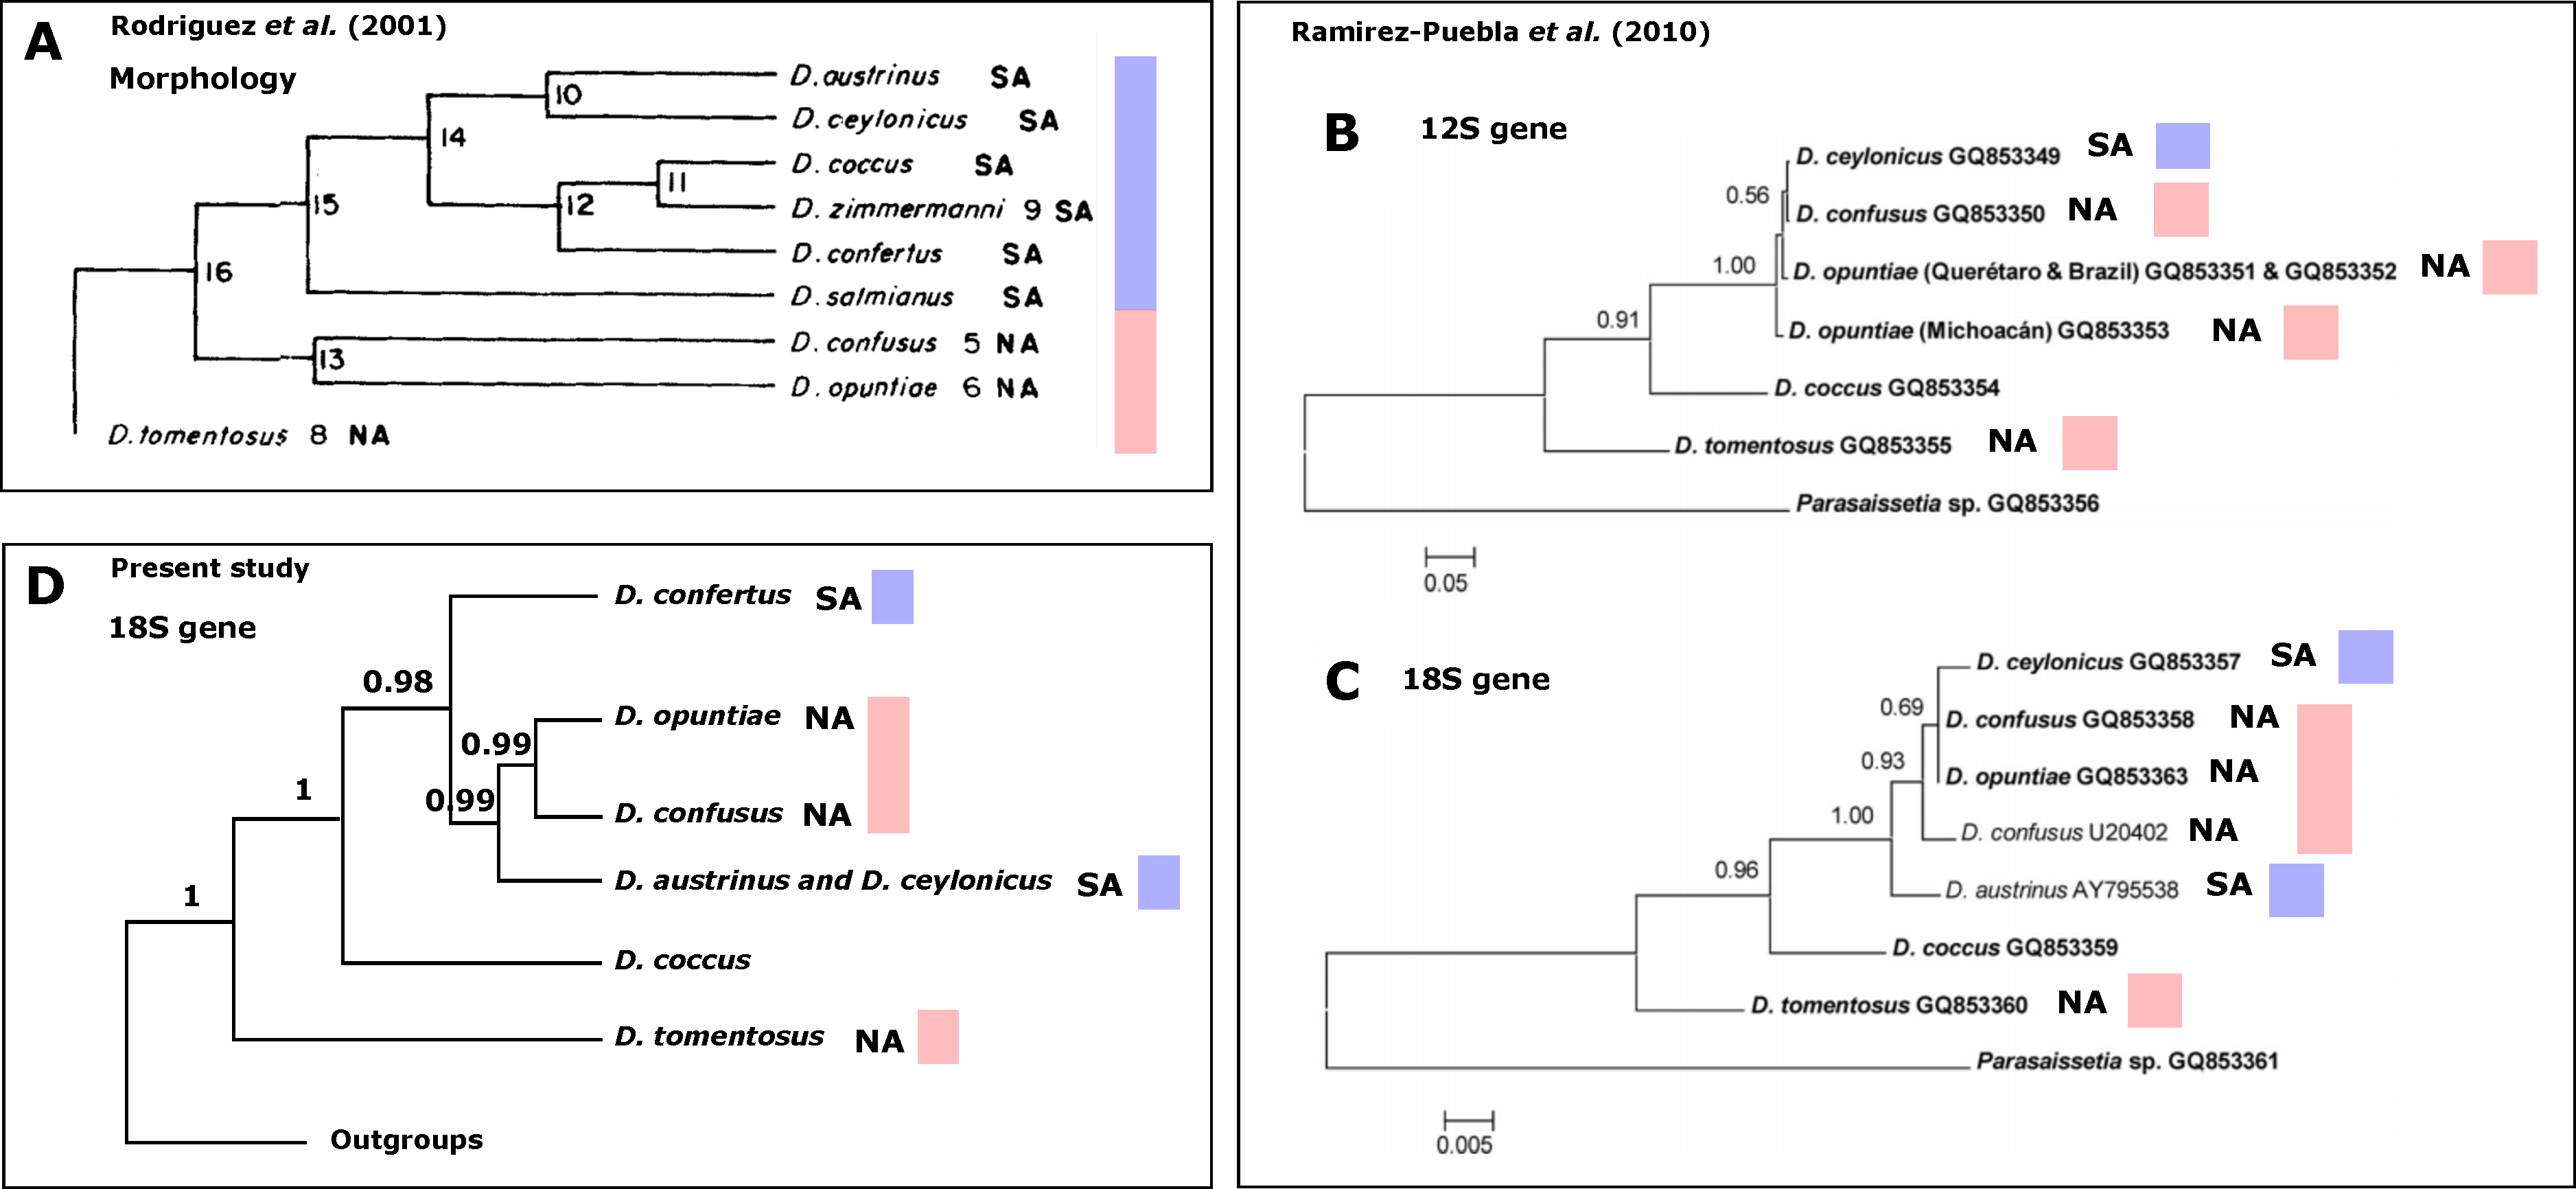
\includegraphics[scale =0.38]{Images/phylogeny_comparison.pdf}
	\caption{A comparison of the phylogenies produced by A) \citet{Rodriguez2001} based on morphological characteristics, \citet{Ramirez-Puebla2010MolecularBacteria} based on the B) 12S and C) 18S rRNA gene regions, and D) the present study, represented as a cladogram for the 18S region (not to scale). The values on the branches of diagrams B, C, and D are Bayesian posterior probability values. NA = North America; SA = South America.} 
	\label{fig:phylogeny_comparison}
\end{figure}

\end{landscape}

\section{Utility of DNA and molecular barcoding}
The barcoding methods used in this study provide a wide range of practical applications for the identification of the Dactylopiidae; particularly for countries such as South Africa and Australia that are the most heavily invaded by invasive cacti. This includes cases such as: 
\vspace{.4cm}

\begin{enumerate}
    \item Identifying potential cryptic species, new lineages, and new species that could be used for the control of invasive Cactaceae in the future.
    \item Identifying hybrids resulting from lineage crosses.
    \item Ensuring that the most effective lineages are present at field sites to enable the highest level of control possible.
    \item Distinguishing pest populations from biocontrol agent populations.
\end{enumerate}

\subsection{New species, cryptic species, and lineages}
Countries such as South Africa and Australia are eager to source and test new agents for controlling target Cactaceae. Both \citet{Paterson2011BiologicalAfrica} and  \citet{jones2016host} point out the potential need for multiple \textit{Dactylopius} lineages to control a diverse range of species. The Dactylopiidae are notoriously difficult to identify, and, as this project has highlighted, taxonomists can sometimes misidentify specimens due to problems with this family's taxonomy and identification keys. DNA and molecular data offers an independent line of evidence for identification, and also provides phylogenetic information about the relationships between species. \\
South Africa is in the process of importing what has been identified as \textit{D. ceylonicus} for the control of \textit{O. elata}, and has recently submitted an application of the release of \textit{
D. tomentosus} `californica var. parkeri' for the control of \textit{C. pallida} (Iain Paterson, pers. comm.). Up to now, the Australians have imported a total of 20 different \textit{D. tomentosus} lineages into quarantine for the potential control of a variety of \textit{Cylindropuntia} species \citep{isbcw2018Jones}. For new agents that have not yet been released, barcoding techniques can be used to confirm their identity prior to release; as they might be completely new species! Having a genetic database to compare new sequences to, as created in this project via the R-based program `Dacty-ID', will make this process quicker and easier. Although DNA barcoding alone is not sufficient to describe a new species, it can certainly be used to earmark potential samples for further investigation.

\subsection{Identifying hybrids}
Intra-specific lineages within the Dactylopiidae are known to hybridise, as discussed in Section \ref{ch01:species_summary}. This directly affects the host specificity of hybrid populations, and thus their virulence. This has important implications in the planning of agent releases; as lineages that produce less damaging hybrid offspring should be kept apart in the field and restricted to the correct target weed species. For example, \citet{Hoffmann2002BiologicalBiotypes} found that \textit{D. opuntiae} `ficus' and `stricta' lineage crosses yielded F1 hybrids that could survive equally well on either \textit{O. ficus-indica} or \textit{O. stricta} (`generalists', as opposed to their true-bred parent `specialists' that could only feed on the one preferred host species), but F2 crosses yielded offspring that contained varying combinations of both specialists and generalists. This could lead to some offspring being unable to survive if they are incompatible with their natal host plant. 
Alternatively, some lineage crosses might result in more effective hybrid offspring. \citet{Mathenge2010a}, for example, found that \textit{D. tomentosus} `cholla' and `imbricata' lineage crosses yielded hybrid offspring that displayed a greater fitness level on their parents' alternative host plant than pure-bred lineages did on the same alternative host species. \\
The dynamics of the hybridisation between other \textit{Dactylopius} lineages are still unknown.
Fragment analysis methods, such as ISSRs, could be a useful identification tool in such future studies.

\subsection{\textit{Dactylopius opuntiae}: pest or biocontrol agent?}
The \textit{Dactylopius opuntiae} `ficus' lineage (the `false
carmine cochineal') has become highly problematic to farmers cultivating \textit{Opuntia ficus-indica} in areas such as Israel, Brazil, Mexico, and Morocco \citep{spodek2014first, cruz2016autonomous, torres2018management}. Some of these areas have reported large-scale financial losses due to the feeding damage caused by this insect. North-eastern Brazil, for example, experienced losses of up to one fifth of cultivated areas valued at some US\$100 million annually \citep{torres2018management, mazzeo2019dactylopius}. Interestingly, one of the proposed hypotheses regarding the introduction and spread of this species in Brazil might also be due to a misidentification. It is postulated that populations of \textit{D. opuntiae} were mistakenly imported instead of \textit{D. coccus} for the creation of a red dye industry \citep{torres2018management}. \\
Having genetic tools to distinguish between what is a pest, and what is a beneficial biocontrol agent (such as the `stricta' lineage, that is not able to survive on \textit{O. ficus-indica} \citep{githure1999host}) can be very useful. Especially since the safety reputation of biological control is at stake. For example, the \textit{D. opuntiae} `stricta' lineage has been released in Saudi Arabia to control \textit{O. stricta}. A pest population of \textit{D. opuntiae} `ficus' is a phytosanitary pest in Israel, and was not introduced as a biocontrol agent. It is important that this pest lineage is not thought to be the same agent released in Saudi Arabia. The `stricta' lineage released in Saudi Arabia is host-specific, and will not feed on cactus crop species.

\section{Conclusion}

This thesis aimed to create multi-locus gene phylogenies for the Dactylopiidae, and to use these data to allow for the quick identification of species and intraspecific lineages. This was achieved through the use of three DNA gene regions and two ISSRs to create a reference database. Before this study, it was not possible to tell the \textit{D. opuntiae} `ficus' and `stricta' lineages apart because they are so genetically similar (and morphologically identical).
% This was done through the use of the 12S, 18S, and COI genetic markers. These enabled accurate identification at the species level, and at the lineage level for most of the \textit{Dactylopius tomentosus} lineages. The two \textit{D. opuntiae} lineages, `stricta' and `ficus', were however indistinguishable from each other. ISSR fragment analysis was subsequently employed to create unique fingerprint profiles for the two groups. The results showed a well-supported separation between them, and population-level differences within the `ficus' lineage. \\
The genetic identification tools arising from this work are important contributions to the biological control of invasive Cactaceae, as the correct identification of control agents is vital to its success. Even different lineages within the same species, and hybrids thereof, can result in different levels of damage to each target weed. \\
The taxonomic history of the Dactylopiidae is riddled with misidentifications, and so a genetic approach is a much-needed addition to the identification toolkit. This can assist in detecting new species, cryptic species, and lineages. It can also be applied to the identification of hybrids arising from lineage crosses. \\
The control of invasive Cactaceae is one of the most successful biological control initiatives in South Africa and Australia, and stands to gain substantially from this streamlined and accurate identification process.
